\chapter{Large Hadron Collider}%%what is it? where is it? why is it?
The Large Hadron Collider (LHC) is a two ring superconducting hadron 
accelerator and collider. It is located on the border of Switzerland
and France to the northwest of the metropolitan area of Geneva.
The LHC is installed in a 26.7 km long tunnel which was originally constructed
from 1984 to 1989 for the Large Electron Positron (LEP) experiment. 
While a hadron hadron collider does not have the same limitations
due to synchroton radiation as an electron positron collider does, %%fix wording
the financial benefits of building the LHC in an existing collider tunnel 
warranted this decision. 
%
%The LHC uses superconducting magnets that operate at 2 K
The LHC is designed to operate at a center of mass energy of 14 TeV.
The overall purpose of constructing a hadron collider with such a high
center of mass energy is to expose the physics beyond the standard model.  

%The LHC is the product of an international collaboration and funded by a large number of country member states.
%%try not to start every sentence with "THE LHC"
\section{Layout}
The LHC follows the LEP tunnel geometry,
a schematic layout of the LHC is shown in figure \ref{fig:LHCring}.
The tunnel is 2.7 m in diameter and houses a twin-bore magnet 
which provides both rings in the same structure.
As can be seen in figure \ref{fig:LHCring},
the LHC can be schematically divided 
into 8 octants. At the center of each octant is a straight section and between
each of the 8 straight section there are 8 arcs. Each straight section
is 528 m long and can serve as an experimental point, where a beam
crossing occurs or as a utility insertion point.
\begin{figure}[t]
  \centering
	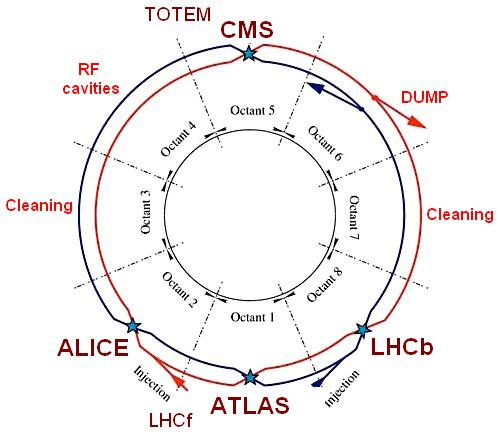
\includegraphics[width=0.6\textwidth]{images/LHCring.jpg}
  	\caption[LHCring]
   	{LHC Experimental and Utility Insertion Layout}
	\label{fig:LHCring}
\end{figure}
ATLAS and CMS are both high luminosity experiments;
the ATLAS experiment is located at Point 1 and, on the opposite side
of the ring, CMS is located at Point 5. 
%%some info about LHCb and ALICE
% the LHC-B experiment at Point 2, ALICE experiment is at Point 8. 
Located at points 3 and 7 are collimation systems for beam cleaning,
the beam dump is at point 6 and point 4 contains to RF systems.

Each of the arcs that stretch between the straight sections
are made of 23 arc cells. Each arc cell is 106.9 m in length
and is comprised of two half cells each of which are 53.45 m long.

\section{Performance Goals and Constraints}
The purpose of the LHC is to be
capable of exposing physics processes that are beyond the standard
model. This can be achieved with beams %%fix wording
that have both high energies and high intensities.
The number of events, N, delivered per second as a function
of machine luminosity, L, is,
\begin{equation}
N=L\sigma_{event}
\end{equation}
where $\sigma_{event}$ is the cross section of the event.
The machine luminosity itself depends on the beam parameters,
\begin{equation}
L=\frac{N_{b}^{2}n_{b}f_{rev}\gamma_{r}}{4\pi \epsilon_{n}\beta^{*}}F
\end{equation}
Here, $N_{b}$ is the number of particles per bunch, $n_{b}$
is the number of bunches per beam, $f_{rev}$ is the
revolution frequency, $\gamma_{r}$ is the relativistic factor, 
$\epsilon_{n}$ is the normalized transverse beam
emittance, $\beta^{*}$ is the a function of the collision point
and F is the geometric luminosity reduction factor due to the crossing
angle at the collision point. 

A number of factors constrain the luminosity that the LHC is capable
of delivering: $N_{b}/\epsilon_{n}$ is limited by the%%new paragraph?
non-linear beam interaction that occurs when beams collide. This
beam-beam interaction is measured by a linear tune shift, $\xi$, where,
\begin{equation}
%write in equation
\end{equation}
Data from previous hadron colliders show that when summed over
all IPs $\xi$ should not exceed 0.015. %new paragraph?
Futhermore, the 
The transverse beam emittance $\epsilon_{n}$
%Beam-Beam Limit
%Mechanical Aperture
%Energy stored in the circulating beams and in magnetic fields
%Heat Load
%Magnets
To collide two counter-rotating proton beams requires magnetic fields
with opposite dipoles. Due to the space constraint in the LEP/LHC
tunnel twin bore magnets are used that consist of two sets of 
two sets of coils and beam channels within the same structure and
sharing the same cooling. 

\section{Operation}
%RF System

\section{Operating Conditions in 2011 and 2012}

